\documentclass{article}
\usepackage[utf8x]{inputenc}
% \usepackage[english,hebrew]{babel}
% \selectlanguage{English}
\usepackage[top=2cm,bottom=2cm,left=2.5cm,right=2cm]{geometry}
\usepackage{amssymb}
\usepackage{amsmath}
\usepackage{cancel}
\usepackage{graphicx}
\usepackage{tabularx}
\usepackage{parcolumns,lipsum}
\usepackage{tikz}
\usetikzlibrary{shapes,positioning}
\title{Ex1 | Introduction to Networks}
\author{Eran Ston (206704512) \and Oded Vaalany (208230474)}
\date{\today}

\begin{document}

\maketitle

\section{Question 1}
Given the following network graph:
\begin{figure}[h]
    \centering
    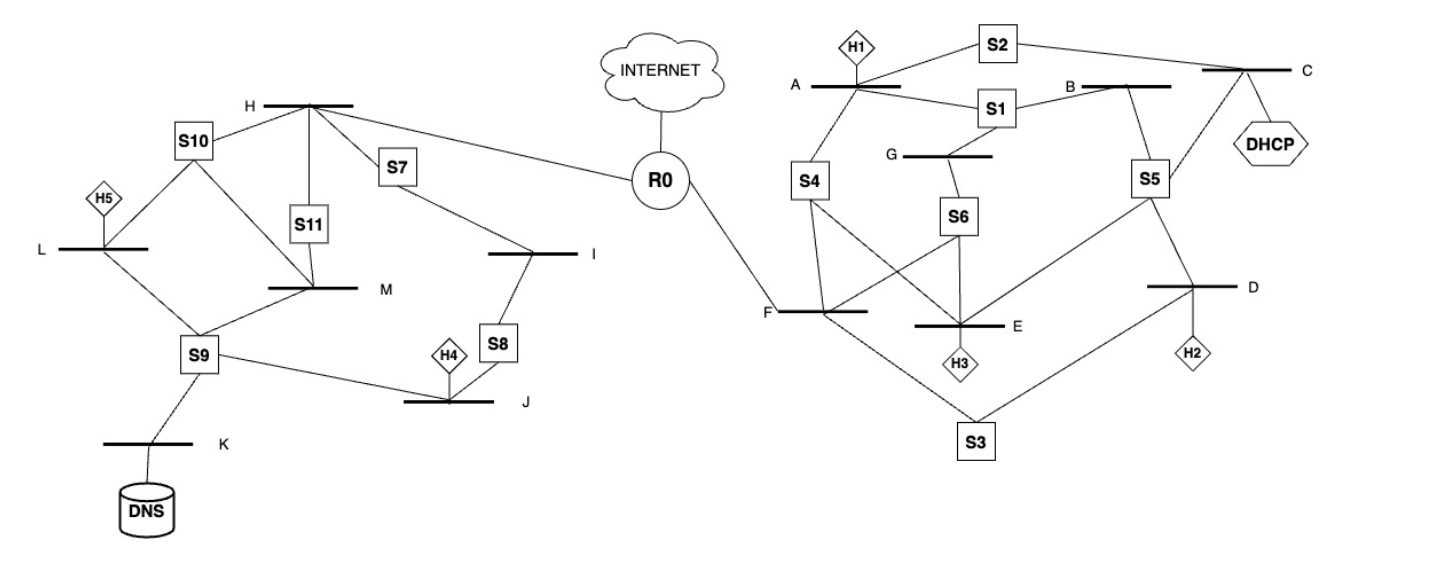
\includegraphics[width=0.9\textwidth]{question1.png}
\end{figure}

\subsection{The end unit H5 connects to the left network. Within it LAN there is noe DHCP server explain how the end unit H5 can get an IP address automaticlly.}
\subsubsection{Elaborate on the needed configuration such the end unit H5 will be able to get an IP address automatically.}

Firstly we need to configure R0 to transfer DHCP requests to the other network. and vice versa.

\subsubsection{named the massages that are used when H5 connects and request an IP address.}

\begin{itemize}
    \item DHCP Discover in the left network.
    \item R0 forwards the DHCP Discover to the right network.
    \item DHCP Offer in the right network.
    \item R0 forwards the DHCP Offer to the left network.
    \item DHCP Request in the left network.
    \item R0 forwards the DHCP Request to the right network.
    \item DHCP Ack in the right network.
    \item R0 forwards the DHCP Ack to the left network.
    \item DHCP Ack in the left network.
\end{itemize}
\subsection{Let's assume that unit H3 activated for the first time, and it want to send one massage to www.huji.ac.il (IP: 123.4.5.6) in the internet. Fill the table with all the massages sends. }
\begin{tabular}{|p{0.05\linewidth}|c|c|p{0.1\linewidth}|p{0.1\linewidth}|p{0.05\linewidth}|p{0.15\linewidth}|p{0.15\linewidth}|}
    \hline
    The network & Source IP & Destination IP & Source MAC & Destination MAC & Pro-tocol & Massage Type & Explain \\
    \hline
    Right & 0.0.0.0 & 255.255.255.255 & H3 & Brodcast & DHCP & DHCP Discover & BC3 \\
    \hline
    Right & DHCP & 255.255.255.255 & DHCP & Brodcast & DHCP & DHCP Offer & BC3 \\
    \hline
    Right & 0.0.0.0 & 255.255.255.255 & H3 & Brodcast & DHCP & DHCP Request & BC3 \\
    \hline
    Right & DHCP & 255.255.255.255 & DHCP & Brodcast & DHCP & DHCP ACK & BC3 \\
    \hline
    Right & - & - & H3 & R0(1) & ARP & ARP Request - DNS Server & -\\
    \hline
    Left & - & - & R0(2) & Brodcast & ARP & ARP Request - H3 & transfer the request for H3 \\    
    \hline
    Left & - & - & DNS & R0(2) & ARP & ARP Response - DNS Server & R0 will transfer this \\
    \hline
    Right & - & - & R0(1) & H3 & ARP & ARP Response - DNS Server & - \\
    \hline
    Right & H3 & DNS & H3 & R0(1) & DNS & DNS Request - www.huji.ac.il & -\\
    \hline
    Left & H3 & DNS & R0(2) & DNS & DNS & DNS Request - www.huji.ac.il &  -\\
    \hline
    Left & DNS & H3 & DNS & R0(2) & DNS & DNS Response - www.huji.ac.il & - \\
    \hline
    Right & DNS & H3 & R0(1) & H3 & DNS & DNS Response - www.huji.ac.il & - \\
    \hline
    Right & H3 & 123.4.5.6 & H3 & R0(1) & HTTP & HTTP Request - www.huji.ac.il & - \\
    \hline
    Right & 123.4.5.6 & H3 & R0(1) & H3 & HTTP & HTTP Response - www.huji.ac.il & - \\
    \hline
\end{tabular}
\section{Question 2}
The parts in this questions are not depends on each other.
\subsection{Part 1}
\subsubsection{subquestion 1}
\begin{itemize}
    \item Host send Request to local DNS server.
    \item Local DNS server send Request to Root DNS server.
    \item Root DNS server Response to Local DNS server the location of '.com' DNS server.
    \item Local DNS server send Request to '.com' DNS server.
    \item '.com' DNS server Response to Local DNS server the location of `ns1.drekflix.com' DNS server.
    \item Local DNS server send Request for `movies.local.drekflix.com' from `ns1.drekflix.com' DNS server.
    \item `ns1.drekflix.com' DNS server Response to Local DNS server the IP address of `ns1.israel.drekflix.com'.
    \item Local DNS server send Request for `movies.local.drekflix.com' from `ns1.israel.drekflix.com' DNS server.
    \item `ns1.israel.drekflix.com' DNS server Response to Local DNS server the IP address of `movies.local.drekflix.com'.
    \item Local DNS server send Response to Host with the IP address of `movies.local.drekflix.com'.
\end{itemize}

\subsubsection{subquestion 2}
When one DNS server received a response from another DNS server and update the response in it chache, the TTL ot this records define by the response DNS server as the Authorative DNS server.
\subsubsection{subquestion 3}

`ns1.israel.drekflix.com' wants to be a load-balancing dns server and therefore it crucial to have a short TTL. The reason is that if the IP address of the server changes, the DNS server needs to update the records in the local DNS resolvers. If the TTL is long, the local DNS resolvers will not update the records and the traffic will not be balanced between the servers.
the other dns servers can have a long TTL since they are not the load-balancing servers and the IP address of the servers is not changed frequently.

so we will receive the following TTLs:
\begin{itemize}
    \item Root DNS server: return records with TTL in days.
    \item '.com' DNS server: return records with TTL in days.
    \item `ns1.drekflix.com': return records with TTL in days.
    \item `ns1.israel.drekflix.com': return records with TTL in minutes.
    \end{itemize}

\subsection{Part 2}


\subsubsection{subquestion 1}
Since there were a storm that cause dammage to the main DNS server, the DNS server is not available. The DNS server is the one that responsible for the domain '.mad'. And even tho the Server who host the domain `www.brass-monkey-saloon.mad' in order to resolve this address the Local DNS resolver needs first to resolve the domain '.mad'. Since the main DNS server is not available the Local DNS resolver can't resolve the domain '.mad' and therefore can't resolve the domain `www.brass-monkey-saloon.mad'. 
\subsubsection{subquestion 2}
The reasone why it takes time after the DNS server dammage until the traffic in Madripor failed is because the cached domain in the local DNS resolvers. The TTL of the records in the local DNS resolvers is not expired yet, and therefore the local DNS resolvers can still resolve the domains end with '.mad'. Since the resolvers are probabliy local and the storme dammage hit far away from the country, the local DNS resolvers can still resolve the domains. 

The time it takes until the traffic in Madripor failed is the time it takes until the TTL of the records in the local DNS resolvers expired.
\section{Question 3}

In Distance Vector Protocol we will split the time to synced time units between all vertexes donates as $t1, t2, t3,\dots$ 
\begin{itemize}
    \item In each time unit $t_i$ each vertex that needs do those steps:
    \begin{itemize}
        \item Send the distance vector to all neighbors.
            \item Receive the distance vector that sent to him.
            \item Update its distance vector.
    \end{itemize}           
    \item In Addition, when the weight of an edge changes, the connected vertexes will update their distance vector in the next time unit.
\end{itemize}
Given the following graph: \\
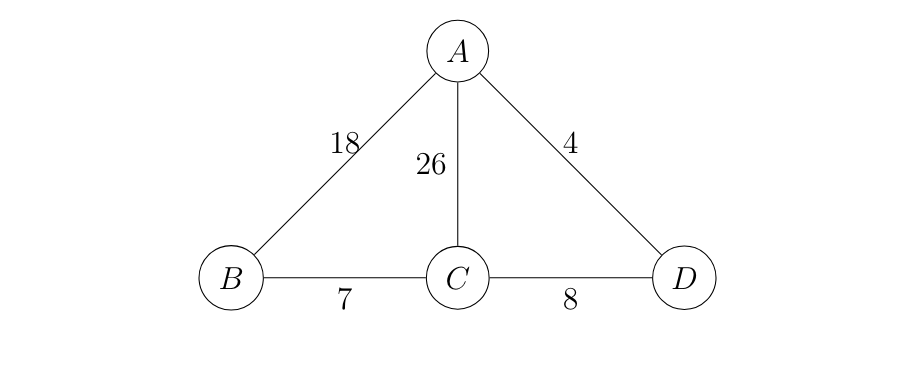
\includegraphics[width=0.9\textwidth]{Screenshot 2024-06-28 at 14.59.41.png}

\subsection{Subquestion 1}
assume that the net is stable for $t_0$ and all the distance vectors are updated.
we made a change in edge AB from 18 to 1. we will show the distance vectors of all the vertexes in the $t_1,t_2$\\



\begin{tabular}{p{0.4\linewidth} p{0.1\linewidth} p{0.4\linewidth}}

    This is the distance vectors of all the vertexes in the $t_0$: & & When the weight of the edge AB changes to 1, A,B imidiately update their distance vector and will send them in the next time unit $t_1$. Therefore this will be the effect on the changes\\
\begin{tabular}{c|c|c|c|c}
    \hline
    Node A & A & B & C & D \\
    \hline
    A & 0 & 18 & 12 & 4 \\
    B & 18 & 0 & 7 & 15 \\
    C & 12 & 7 & 0 & 8 \\
    D & 4 & 15 & 8 & 0 \\
    \hline
    \hline
    Node B & A & B & C & D \\
    \hline 
    A & 0 & 18 & 12 & 4 \\
    B & 18 & 0 & 7 & 15 \\
    C & 12 & 7 & 0 & 8 \\
    \hline
    \hline
    Node C & A & B & C & D \\
    \hline
    A & 0 & 18 & 12 & 4 \\
    B & 18 & 0 & 7 & 15 \\
    C & 12 & 7 & 0 & 8 \\
    D & 4 & 15 & 8 & 0 \\
    \hline
    \hline
    Node D & A & B & C & D \\
    \hline
    A & 0 & 18 & 12 & 4 \\
    C & 12 & 7 & 0 & 8 \\
    D & 4 & 15 & 8 & 0 \\
    \hline
\end{tabular}
& \centering $\Rightarrow$&
    \begin{tabular}{c|c|c|c|c}
        \hline
        Node A & A & B & C & D \\
        \hline
        A & 0 & \color{red}1 & \color{red}8 & 4 \\
        B & 18 & 0 & 7 & 15 \\
        C & 12 & 7 & 0 & 8 \\
        D & 4 & 15 & 8 & 0 \\
        \hline
        \hline
        Node B & A & B & C & D \\
        \hline 
        A & 0 & 18 & 12 & 4 \\
        B & \color{red}1 & 0 & 7 & \color{red}5 \\
        C & 12 & 7 & 0 & 8 \\
        \hline
        \hline
        Node C & A & B & C & D \\
        \hline
        A & 0 & 18 & 12 & 4 \\
        B & 18 & 0 & 7 & 15 \\
        C & 12 & 7 & 0 & 8 \\
        D & 4 & 15 & 8 & 0 \\
        \hline
        \hline
        Node D & A & B & C & D \\
        \hline
        A & 0 & 18 & 12 & 4 \\
        C & 12 & 7 & 0 & 8 \\
        D & 4 & 15 & 8 & 0 \\
        \hline
    \end{tabular}
\end{tabular}

\textbf{Now we will show the before and after with time unit $t_1$}\\
\begin{tabular}{p{0.4\linewidth} p{0.1\linewidth} p{0.4\linewidth}}
    After receiving the distance vectors from the neighbors &  & End of $t_1$ \\
    \begin{tabular}{c|c|c|c|c}
        \hline
        Node A & A & B & C & D \\
        \hline
        A & 0 & \color{red}1 & \color{red}8 & 4 \\
        B & \color{red}1 & 0 & 7 & \color{red}5 \\
        C & 12 & 7 & 0 & 8 \\
        D & 4 & 15 & 8 & 0 \\
        \hline
        \hline
        Node B & A & B & C & D \\
        \hline 
        A & 0 & \color{red}1 & \color{red}8 & 4 \\
        B & \color{red}1 & 0 & 7 & \color{red}5 \\
        C & 12 & 7 & 0 & 8 \\
        \hline
        \hline
        Node C & A & B & C & D \\
        \hline
        A & 0 & \color{red}1 & \color{red}8 & 4 \\
        B & \color{red}1 & 0 & 7 & \color{red}5 \\
        C & 12 & 7 & 0 & 8 \\
        D & 4 & 15 & 8 & 0 \\
        \hline
        \hline
        Node D & A & B & C & D \\
        \hline
        A & 0 & \color{red}1 & \color{red}8 & 4 \\
        C & 12 & 7 & 0 & 8 \\
        D & 4 & 15 & 8 & 0 \\
        \hline
    \end{tabular}
    & \centering $\Rightarrow$&

    \begin{tabular}{c|c|c|c|c}
        \hline
        Node A & A & B & C & D \\
        \hline
        A & 0 & 1 & 8 & 4 \\
        B & 1 & 0 & 7 & 5 \\
        C & 12 & 7 & 0 & 8 \\
        D & 4 & 15 & 8 & 0 \\
        \hline
        \hline
        Node B & A & B & C & D \\
        \hline 
        A & 0 & 1 & 8 & 4 \\
        B & 1 & 0 & 7 & 5 \\
        C & 12 & 7 & 0 & 8 \\
        \hline
        \hline
        Node C & A & B & C & D \\
        \hline
        A & 0 & 1 & 8 & 4 \\
        B & 1 & 0 & 7 & 5 \\
        C & \color{red}8 & 7 & 0 & 8 \\
        D & 4 & 15 & 8 & 0 \\
        \hline
        \hline
        Node D & A & B & C & D \\
        \hline
        A & 0 & 1 & 8 & 4 \\
        C & 12 & 7 & 0 & 8 \\
        D & 4 & \color{red}5 & 8 & 0 \\
        \hline


    \end{tabular}

\end{tabular}\\

\textbf{Now we will show the before and after with time unit $t_2$}\\
\begin{tabular}{p{0.4\linewidth} p{0.1\linewidth} p{0.4\linewidth}}
    After Receiving the distance vectors from the neighbors &  & End of $t_2$ \\
    \begin{tabular}{c|c|c|c|c}
        \hline
        Node A & A & B & C & D \\
        \hline
        A & 0 & 1 & 8 & 4 \\
        B & 1 & 0 & 7 & 5 \\
        C & \color{red}8 & 7 & 0 & 8 \\
        D & 4 & \color{red}5 & 8 & 0 \\
        \hline
        \hline
        Node B & A & B & C & D \\
        \hline 
        A & 0 & 1 & 8 & 4 \\
        B & 1 & 0 & 7 & 5 \\
        C & \color{red}8 & 7 & 0 & 8 \\
        \hline
        \hline
        Node C & A & B & C & D \\
        \hline
        A & 0 & 1 & 8 & 4 \\
        B & 1 & 0 & 7 & 5 \\
        C & 8 & 7 & 0 & 8 \\
        D & 4 & \color{red}5 & 8 & 0 \\
        \hline
        \hline
        Node D & A & B & C & D \\
        \hline
        A & 0 & 1 & 8 & 4 \\
        C & \color{red}8 & 7 & 0 & 8 \\
        D & 4 & 5 & 8 & 0 \\
        \hline
    \end{tabular}
    & \centering $\Rightarrow$&
    \begin{tabular}{c|c|c|c|c}
        \hline
        Node A & A & B & C & D \\
        \hline
        A & 0 & 1 & 8 & 4 \\
        B & 1 & 0 & 7 & 5 \\
        C & 8 & 7 & 0 & 8 \\
        D & 4 & 5 & 8 & 0 \\
        \hline
        \hline
        Node B & A & B & C & D \\
        \hline 
        A & 0 & 1 & 8 & 4 \\
        B & 1 & 0 & 7 & 5 \\
        C & 8 & 7 & 0 & 8 \\
        \hline
        \hline
        Node C & A & B & C & D \\
        \hline
        A & 0 & 1 & 8 & 4 \\
        B & 1 & 0 & 7 & 5 \\
        C & 8 & 7 & 0 & 8 \\
        D & 4 & 5 & 8 & 0 \\
        \hline
        \hline
        Node D & A & B & C & D \\
        \hline
        A & 0 & 1 &  8 & 4 \\
        C & 8 & 7 & 0 & 8 \\
        D & 4 & 5 & 8 & 0 \\
        \hline
    \end{tabular}


\end{tabular}

\subsection{Subquestion 2}
Now the edge CD changes from 8 to 32. we will show the distance vectors of all the vertexes in the $t_1,t_2,t_3$\\
\newline
\begin{tabular}{p{0.4\linewidth} p{0.1\linewidth} p{0.4\linewidth}}

    This is the distance vectors of all the vertexes in the $t_0$: &  & When the weight of the edge DC changes to 32, D,C imidiately update their distance vector and will send them in the next time unit $t_1$. Therefore this will be the effect on the changes\\
\begin{tabular}{c|c|c|c|c}
    \hline
    Node A & A & B & C & D \\
    \hline
    A & 0 & 18 & 12 & 4 \\
    B & 18 & 0 & 7 & 15 \\
    C & 12 & 7 & 0 & 8 \\
    D & 4 & 15 & 8 & 0 \\
    \hline
    \hline
    Node B & A & B & C & D \\
    \hline 
    A & 0 & 18 & 12 & 4 \\
    B & 18 & 0 & 7 & 15 \\
    C & 12 & 7 & 0 & 8 \\
    \hline
    \hline
    Node C & A & B & C & D \\
    \hline
    A & 0 & 18 & 12 & 4 \\
    B & 18 & 0 & 7 & 15 \\
    C & 12 & 7 & 0 & 8 \\
    D & 4 & 15 & 8 & 0 \\
    \hline
    \hline
    Node D & A & B & C & D \\
    \hline
    A & 0 & 18 & 12 & 4 \\
    C & 12 & 7 & 0 & 8 \\
    D & 4 & 15 & 8 & 0 \\
    \hline
\end{tabular}
& \centering $\Rightarrow$&
\begin{tabular}{c|c|c|c|c}
    \hline
    Node A & A & B & C & D \\
    \hline
    A & 0 & 18 & 12 & 4 \\
    B & 18 & 0 & 7 & 15 \\
    C & 12 & 7 & 0 & 8 \\
    D & 4 & 15 & 8 & 0 \\
    \hline
    \hline
    Node B & A & B & C & D \\
    \hline 
    A & 0 & 18 & 12 & 4 \\
    B & 18 & 0 & 7 & 15 \\
    C & 12 & 7 & 0 & 8 \\
    \hline
    \hline
    Node C & A & B & C & D \\
    \hline
    A & 0 & 18 & 12 & 4 \\
    B & 18 & 0 & 7 & 15 \\
    C & \color{red}25 & 7 & 0 & \color{red}22 \\
    D & 4 & 15 & 8 & 0 \\
    \hline
    \hline
    Node D & A & B & C & D \\
    \hline
    A & 0 & 18 & 12 & 4 \\
    C & 12 & 7 & 0 & 8 \\
    D & 4 & \color{red}22 & \color{red}16 & 0 \\
    \hline
\end{tabular}
\end{tabular}
\newline
\textbf{Now we will show the before and after with time unit $t_1$}\\
\newline

\begin{tabular}{p{0.4\linewidth} p{0.1\linewidth} p{0.4\linewidth}}

    After Receiving the distance vectors from the
    neighbors &  & End of $t_1$ \\
\begin{tabular}{c|c|c|c|c}
    \hline
    Node A & A & B & C & D \\
    \hline
    A & 0 & 18 & 12 & 4 \\
    B & 18 & 0 & 7 & 15 \\
    C & \color{red}25 & 7 & 0 & \color{red}22 \\
    D & 4 & \color{red}22 & \color{red}16 & 0 \\
    \hline
    \hline
    Node B & A & B & C & D \\
    \hline 
    A & 0 & 18 & 12 & 4 \\
    B & 18 & 0 & 7 & 15 \\
    C & \color{red}25 & 7 & 0 & \color{red}22 \\
    \hline
    \hline
    Node C & A & B & C & D \\
    \hline
    A & 0 & 18 & 12 & 4 \\
    B & 18 & 0 & 7 & 15 \\
    C & 25 & 7 & 0 & 22 \\
    D & 4 & \color{red}22 & \color{red}16 & 0 \\
    \hline
    \hline
    Node D & A & B & C & D \\
    \hline
    A & 0 & 18 & 12 & 4 \\
    C & \color{red}25 & 7 & 0 & \color{red}22 \\
    D & 4 & \color{red}22 & \color{red}16 & 0 \\
    \hline
\end{tabular}
& \centering $\Rightarrow$&
\begin{tabular}{c|c|c|c|c}
    \hline
    Node A & A & B & C & D \\
    \hline
    A & 0 & 18 & \color{red}20 & 4 \\
    B & 18 & 0 & 7 & 15 \\
    C & 25 & 7 & 0 & 22 \\
    D & 4 & 22 & 16 & 0 \\
    \hline
    \hline
    Node B & A & B & C & D \\
    \hline 
    A & 0 & 18 & 12 & 4 \\
    B & 18 & 0 & 7 & \color{red}22 \\
    C & 25 & 7 & 0 & 22 \\
    \hline
    \hline
    Node C & A & B & C & D \\
    \hline
    A & 0 & 18 & 12 & 4 \\
    B & 18 & 0 & 7 & 15 \\
    C & 25 & 7 & 0 & \color{red}30 \\
    D & 4 & 22 & 16 & 0 \\
    \hline
    \hline
    Node D & A & B & C & D \\
    \hline
    A & 0 & 18 & 12 & 4 \\
    C & 25 & 7 & 0 & 22 \\
    D & 4 & 22 & 16 & 0 \\
    \hline
\end{tabular}
\end{tabular}

\textbf{Now we will show the before and after with time unit $t_2$}\\
\newline

\begin{tabular}{p{0.4\linewidth} p{0.1\linewidth} p{0.4\linewidth}}

    After Receiving the distance vectors from the
    neighbors &  & End of $t_2$ \\
    \begin{tabular}{c|c|c|c|c}
        \hline
        Node A & A & B & C & D \\
        \hline
        A & 0 & 18 & \color{red}20 & 4 \\
        B & 18 & 0 & 7 & \color{red}22 \\
        C & 25 & 7 & 0 & \color{red}30 \\
        D & 4 & 22 & 16 & 0 \\
        \hline
        \hline
        Node B & A & B & C & D \\
        \hline 
        A & 0 & 18 & \color{red}20 & 4 \\
        B & 18 & 0 & 7 & \color{red}22 \\
        C & 25 & 7 & 0 & \color{red}30 \\
        \hline
        \hline
        Node C & A & B & C & D \\
        \hline
        A & 0 & 18 & \color{red}20 & 4 \\
        B & 18 & 0 & 7 & \color{red}22 \\
        C & 25 & 7 & 0 & \color{red}30 \\
        D & 4 & 22 & 16 & 0 \\
        \hline
        \hline
        Node D & A & B & C & D \\
        \hline
        A & 0 & 18 & \color{red}20 & 4 \\
        C & 25 & 7 & 0 & \color{red}30 \\
        D & 4 & 22 & 16 & 0 \\
        \hline
    \end{tabular}
& \centering $\Rightarrow$&
\begin{tabular}{c|c|c|c|c}
    \hline
    Node A & A & B & C & D \\
    \hline
    A & 0 & 18 & 20 & 4 \\
    B & 18 & 0 & 7 & 22 \\
    C & 25 & 7 & 0 & 30 \\
    D & 4 & 22 & 16 & 0 \\
    \hline
    \hline
    Node B & A & B & C & D \\
    \hline 
    A & 0 & 18 & 20 & 4 \\
    B & 18 & 0 & 7 & 22 \\
    C & 25 & 7 & 0 & 30 \\
    \hline
    \hline
    Node C & A & B & C & D \\
    \hline
    A & 0 & 18 & 20 & 4 \\
    B & 18 & 0 & 7 & 22 \\
    C & 25 & 7 & 0 & \color{red}29 \\
    D & 4 & 22 & 16 & 0 \\
    \hline
    \hline
    Node D & A & B & C & D \\
    \hline
    A & 0 & 18 & 20 & 4 \\
    C & 25 & 7 & 0 & 30 \\
    D & 4 & 22 & \color{red}24 & 0 \\
    \hline
\end{tabular}
\end{tabular}

\textbf{Now we will show the before and after with time unit $t_3$}\\
\newline

\begin{tabular}{p{0.4\linewidth} p{0.1\linewidth} p{0.4\linewidth}}

    After Receiving the distance vectors from the
    neighbors &  & End of $t_3$ \\
    \begin{tabular}{c|c|c|c|c}
        \hline
        Node A & A & B & C & D \\
        \hline
        A & 0 & 18 & 20 & 4 \\
        B & 18 & 0 & 7 & 22 \\
        C & 25 & 7 & 0 & \color{red}29 \\
        D & 4 & 22 & \color{red}24 & 0 \\
        \hline
        \hline
        Node B & A & B & C & D \\
        \hline 
        A & 0 & 18 & 20 & 4 \\
        B & 18 & 0 & 7 & 22 \\
        C & 25 & 7 & 0 & \color{red}29 \\
        \hline
        \hline
        Node C & A & B & C & D \\
        \hline
        A & 0 & 18 & 20 & 4 \\
        B & 18 & 0 & 7 & 22 \\
        C & 25 & 7 & 0 & \color{red}29 \\
        D & 4 & 22 & \color{red}24 & 0 \\
        \hline
        \hline
        Node D & A & B & C & D \\
        \hline
        A & 0 & 18 & 20 & 4 \\
        C & 25 & 7 & 0 & \color{red}29 \\
        D & 4 & 22 & \color{red}24 & 0 \\
        \hline
    \end{tabular}
& \centering $\Rightarrow$&
\begin{tabular}{c|c|c|c|c}
    \hline
    Node A & A & B & C & D \\
    \hline
    A & 0 & 18 & \color{red}25 & 4 \\
    B & 18 & 0 & 7 & 22 \\
    C & 25 & 7 & 0 & 29 \\
    D & 4 & 22 & 24 & 0 \\
    \hline
    \hline
    Node B & A & B & C & D \\
    \hline 
    A & 0 & 18 & 20 & 4 \\
    B & 18 & 0 & 7 & 22 \\
    C & 25 & 7 & 0 & 29 \\
    \hline
    \hline
    Node C & A & B & C & D \\
    \hline
    A & 0 & 18 & 20 & 4 \\
    B & 18 & 0 & 7 & 22 \\
    C & 25 & 7 & 0 & 29 \\
    D & 4 & 22 & 24 & 0 \\
    \hline
    \hline
    Node D & A & B & C & D \\
    \hline
    A & 0 & 18 & 20 & 4 \\
    C & 25 & 7 & 0 & 29 \\
    D & 4 & 22 & 24 & 0 \\
    \hline
\end{tabular}
\end{tabular}

\subsection{subquestion 3}
Now we will show the run using the poisoned reverse technique.\\

\begin{tabular}{p{0.4\linewidth} p{0.1\linewidth} p{0.4\linewidth}}
    The DV before the change & $t_0$ & The DV after the change \\
    \begin{tabular}{c|c|c|c|c}
        \hline
        Node A & A & B & C & D \\
        \hline
        A & 0 & 18 & 12 & 4 \\
        B & 18 & 0 & 7 & 15 \\
        C & 12 & 7 & 0 & 8 \\
        D & 4 & 15 & 8 & 0 \\
        \hline
        \hline
        Node B & A & B & C & D \\
        \hline 
        A & 0 & 18 & 12 & 4 \\
        B & 18 & 0 & 7 & 15 \\
        C & 12 & 7 & 0 & 8 \\
        \hline
        \hline
        Node C & A & B & C & D \\
        \hline
        A & 0 & 18 & 12 & 4 \\
        B & 18 & 0 & 7 & 15 \\
        C & 12 & 7 & 0 & 8 \\
        D & 4 & 15 & 8 & 0 \\
        \hline
        \hline
        Node D & A & B & C & D \\
        \hline
        A & 0 & 18 & 12 & 4 \\
        C & 12 & 7 & 0 & 8 \\
        D & 4 & 15 & 8 & 0 \\
        \hline
    \end{tabular}
    &  $\Rightarrow$&
    \begin{tabular}{c|c|c|c|c}
        \hline
        Node A & A & B & C & D \\
        \hline
        A & 0 & 18 & 12 & 4 \\
        B & 18 & 0 & 7 & 15 \\
        C & 12 & 7 & 0 & 8 \\
        D & 4 & 15 & 8 & 0 \\
        \hline
        \hline
        Node B & A & B & C & D \\
        \hline 
        A & 0 & 18 & 12 & 4 \\
        B & 18 & 0 & 7 & 15 \\
        C & 12 & 7 & 0 & 8 \\
        \hline
        \hline
        Node C & A & B & C & D \\
        \hline
        A & 0 & 18 & 12 & 4 \\
        B & 18 & 0 & 7 & \color{red}$\infty$ \\
        C & \color{red}25 & 7 & 0 & \color{red}30 \\
        D & 4 & 15 & 8 & 0 \\
        \hline
        \hline
        Node D & A & B & C & D \\
        \hline
        A & 0 & 18 & \color{red}$\infty$ & 4 \\
        C & 12 & 7 & 0 & 8 \\
        D & 4 & \color{red}22 & \color{red}32 & 0 \\
        \hline
    \end{tabular} \\ \\ \\ 

    The DV after the change & $t_1$ & The DV after the change \\
    \begin{tabular}{c|c|c|c|c}
        \hline
        Node A & A & B & C & D \\
        \hline
        A & 0 & 18 & 12 & 4 \\
        B & 18 & 0 & 7 & 15 \\
        C & \color{red}25 & 7 & 0 & \color{red}30 \\
        D & 4 & \color{red}22 & \color{red}32 & 0 \\
        \hline
        \hline
        Node B & A & B & C & D \\
        \hline 
        A & 0 & 18 & 12 & 4 \\
        B & 18 & 0 & 7 & 15 \\
        C & \color{red}25 & 7 & 0 & \color{red}30 \\
        \hline
        \hline
        Node C & A & B & C & D \\
        \hline
        A & 0 & 18 & 12 & 4 \\
        B & 18 & 0 & 7 & $\infty$ \\
        C & \color{red}25 & 7 & 0 & \color{red}30 \\
        D & 4 & \color{red}22 & \color{red}32 & 0 \\
        \hline
        \hline
        Node D & A & B & C & D \\
        \hline
        A & 0 & 18 & $\infty$ & 4 \\
        C & \color{red}25 & 7 & 0 & \color{red}30 \\
        D & 4 & \color{red}22 & \color{red}32 & 0 \\
        \hline
    \end{tabular}
    &  $\Rightarrow$&
    \begin{tabular}{c|c|c|c|c}
        \hline
        Node A & A & B & C & D \\
        \hline
        A & 0 & 18 & \color{red}25 & 4 \\
        B & 18 & 0 & 7 & 15 \\
        C & 25 & 7 & 0 & 30 \\
        D & 4 & 22 & 32 & 0 \\
        \hline
        \hline
        Node B & A & B & C & D \\
        \hline 
        A & 0 & 18 & 12 & 4 \\
        B & 18 & 0 & 7 & \color{red}22 \\
        C & 25 & 7 & 0 & 30 \\
        \hline
        \hline
        Node C & A & B & C & D \\
        \hline
        A & 0 & 18 & 12 & 4 \\
        B & 18 & 0 & 7 & $\infty$ \\
        C & 25 & 7 & 0 & \color{red}30 \\
        D & 4 & 22 & 32 & 0 \\
        \hline
        \hline
        Node D & A & B & C & D \\
        \hline
        A & 0 & 18 & $\infty$ & 4 \\
        C & 25 & 7 & 0 & 30 \\
        D & 4 & 22 & 32 & 0 \\
        \hline
    \end{tabular}
\end{tabular} \\ \\
\begin{tabular}{p{0.4\linewidth} p{0.1\linewidth} p{0.4\linewidth}}

    The DV after the change & $t_2$ & The DV after the change \\
    \begin{tabular}{c|c|c|c|c}
        \hline
        Node A & A & B & C & D \\
        \hline
        A & 0 & 18 & \color{red}25 & 4 \\
        B & 18 & 0 & 7 & \color{red}22 \\
        C & 25 & 7 & 0 & \color{red}30 \\
        D & 4 & 22 & 32 & 0 \\
        \hline
        \hline
        Node B & A & B & C & D \\
        \hline 
        A & 0 & 18 & \color{red}25 & 4 \\
        B & 18 & 0 & 7 & \color{red}22 \\
        C & 25 & 7 & 0 & \color{red}30 \\
        \hline
        \hline
        Node C & A & B & C & D \\
        \hline
        A & 0 & 18 & \color{red}25 & 4 \\
        B & 18 & 0 & 7 & \color{red}22 \\
        C & 25 & 7 & 0 & \color{red}30 \\
        D & 4 & 22 & 32 & 0 \\
        \hline
        \hline
        Node D & A & B & C & D \\
        \hline
        A & 0 & 18 & \color{red}25 & 4 \\
        C & 25 & 7 & 0 & \color{red}30 \\
        D & 4 & 22 & 32 & 0 \\
        \hline
    \end{tabular}
    &  $\Rightarrow$&
    \begin{tabular}{c|c|c|c|c}
        \hline
        Node A & A & B & C & D \\
        \hline
        A & 0 & 18 & 25 & 4 \\
        B & 18 & 0 & 7 & 22 \\
        C & 25 & 7 & 0 & 30 \\
        D & 4 & 22 & 32 & 0 \\
        \hline
        \hline
        Node B & A & B & C & D \\
        \hline 
        A & 0 & 18 & 25 & 4 \\
        B & 18 & 0 & 7 & 22 \\
        C & 25 & 7 & 0 & 30 \\
        \hline
        \hline
        Node C & A & B & C & D \\
        \hline
        A & 0 & 18 & 25 & 4 \\
        B & 18 & 0 & 7 & 22 \\
        C & 25 & 7 & 0 & \color{red}29 \\
        D & 4 & 22 & 32 & 0 \\
        \hline
        \hline
        Node D & A & B & C & D \\
        \hline
        A & 0 & 18 & 25 & 4 \\
        C & 25 & 7 & 0 & 30 \\
        D & 4 & 22 & \color{red}29 & 0 \\
        \hline
    \end{tabular} \\ \\ \\ 
    The DV after the change & $t_3$ & The DV after the change \\
    \begin{tabular}{c|c|c|c|c}
        \hline
        Node A & A & B & C & D \\
        \hline
        A & 0 & 18 & 25 & 4 \\
        B & 18 & 0 & 7 & 22 \\
        C & 25 & 7 & 0 & \color{red}29 \\
        D & 4 & 22 & \color{red}29 & 0 \\
        \hline
        \hline
        Node B & A & B & C & D \\
        \hline 
        A & 0 & 18 & 25 & 4 \\
        B & 18 & 0 & 7 & 22 \\
        C & 25 & 7 & 0 & \color{red}29 \\
        \hline
        \hline
        Node C & A & B & C & D \\
        \hline
        A & 0 & 18 & 25 & 4 \\
        B & 18 & 0 & 7 & 22 \\
        C & 25 & 7 & 0 & \color{red}29 \\
        D & 4 & 22 & \color{red}29 & 0 \\
        \hline
        \hline
        Node D & A & B & C & D \\
        \hline
        A & 0 & 18 & 25 & 4 \\
        C & 25 & 7 & 0 & \color{red}29 \\
        D & 4 & 22 & \color{red}29 & 0 \\
        \hline
    \end{tabular}
    &  $\Rightarrow$&
    \begin{tabular}{c|c|c|c|c}
        \hline
        Node A & A & B & C & D \\
        \hline
        A & 0 & 18 & 25 & 4 \\
        B & 18 & 0 & 7 & 22 \\
        C & 25 & 7 & 0 & 29 \\
        D & 4 & 22 & 29 & 0 \\
        \hline
        \hline
        Node B & A & B & C & D \\
        \hline 
        A & 0 & 18 & 25 & 4 \\
        B & 18 & 0 & 7 & 22 \\
        C & 25 & 7 & 0 & 29 \\
        \hline
        \hline
        Node C & A & B & C & D \\
        \hline
        A & 0 & 18 & 25 & 4 \\
        B & 18 & 0 & 7 & 22 \\
        C & 25 & 7 & 0 & 29 \\
        D & 4 & 22 & 29 & 0 \\
        \hline
        \hline
        Node D & A & B & C & D \\
        \hline
        A & 0 & 18 & 25 & 4 \\
        C & 25 & 7 & 0 & 29 \\
        D & 4 & 22 & 29 & 0 \\
        \hline
    \end{tabular}
\end{tabular}

\subsection{subquestion 4}
No, poisoned reverse does not always solve the count to infinity problem in networking. For example If 
\end{document}